\chapter{Radio Physics}\label{ch:radio-physics}
%\bibtodo{from original report}
The goal of this chapter is to be able to estimate the probability, based on the topology of a wireless
network, of how likely it is that packet loss will happen during a transmission between two nodes.

%\autoref{sec:linkmodel} presents the method for simulating the link model in a \gls{manet}, \autoref{sec:pep}
%presents the method for computing the packet loss probability during a transmission, and
%\autoref{sec:optimization} proposes two ways for optimising the computational time required to compute the
%link model.

\begin{figure}[ht]
    \centering
    \includegraphics[width=.7\textwidth]{figures/manet_with_terrain.png}
    \caption{A wireless network topology.}
    \label{figure:manetwithter}
\end{figure}

\autoref{figure:manetwithter} shows a sample wireless network topology for a \acrfull{manet}. The network
consists of mobile devices (nodes), and the communication between these (links). Nodes are
\doublequote{linked} with other nodes when they are able to communicate wirelessly. Wireless communication
relies on the transmission and reception of electromagnetic waves~\cite[p.~10]{paper:linkmodel} (radio
signals), and the strength, or quality, of a wireless link is described by the signal loss occurring when
propagating the signal from transmitter to receiver, and is measured by the \gls{rssi} (a negative value,
where a value close to 0 is better). In \cite{paper:linkmodel}, the term \gls{pathloss} is used to describe
this signal loss, and is determined in part by the physical distance between transmitter and receiver, but
also by physical objects and terrain, like buildings or forests. A major consideration for mobile networks is
that the topology is dynamic. Nodes move around, causing links to disappear, or new links to appear, thus mast
changing the topology of the network.

%\autoref{sec:linkmodel} will elaborate
%further on the \gls{pathloss} of a link, as well as present a method for simulating the \gls{pathloss} for a
%mobile network topology. 

\section{Visualiser Tool}\label{sec:visualiser}
The Visualiser is a tool written in Python and JavaScript, created by Peter Gjøl Jensen. The tool was created
to aid in visualisation of \gls{manet} topologies, and works by importing a log file with \acrshort{gps}
coordinates and timestamps for a series of nodes. Using the tool, it is possible to visualise the position and
movement for all nodes in a network. A snippet of a \acrshort{gps} log can be seen below. Each line consists
of the identifier of the node, the latitude and longitude coordinates for the node, and the timestamp for the
coordinates in milliseconds.
%
\begin{verbatim}
#id,lat,lon,timestamp
64,14.629879,121.096137,158980000.000000
64,14.629874,121.096132,159000000.000000
64,14.629878,121.096128,159020000.000000
64,14.629890,121.096143,159040000.000000
64,14.629892,121.096142,159060000.000000
64,14.629896,121.096141,159080000.000000
64,14.629893,121.096164,159100000.000000
64,14.629947,121.096083,159120000.000000
64,14.630107,121.095976,159140000.000000
64,14.630283,121.095885,159160000.000000
64,14.630525,121.095786,159180000.000000
\end{verbatim}

\autoref{figure:gpslogvisualised} in \autoref{app:visualiser:screens} shows a screen-shot from the Visualiser,
with a \acrshort{gps} log loaded. When a \acrshort{gps} log is loaded, the Visualiser can be started by
pressing the \doublequote{Play} button, or the \doublequote{space} key. The speed of the visualisation can be
controlled with the \doublequote{Speed} slider in the bottom, and the current time of the visualisation can
be controlled with the \doublequote{Time} slider. 

\subsection{Extensions}
We propose three extension to the visualiser tool. The first is to visualise the link between nodes using an
annotated version of the \acrshort{gps} log, where each line is annotated with the \gls{rssi} of a link
between nodes in the log, as shown below. In the annotated log, each link for a given node, to another node,
is annotated, after the timestamp, with the identifier of the other node, and the \gls{rssi} between them.
\autoref{figure:gpslogrssivisualised} in \autoref{app:visualiser:screens} show an example of a very connected
network where links between nodes are visualised by a colour gradient, where a link with a yellow colour has a
better \gls{rssi} than a link with a red colour. It is possible to print the \gls{rssi} value for the links as
well.
%
\begin{verbatim}
#id,lat,lon,timestamp,id1,rssi1,id2,rssi2,id3,rssi3, ...
65,14.630107,121.096749,157820000.000000,67,-56,69,-70,71,-13, ...
65,14.630129,121.096905,157840000.000000,67,-58,69,-61,73,-65, ...
65,14.630189,121.097116,157860000.000000,67,-55,69,-54,73,-71, ...
65,14.630318,121.097294,157880000.000000,67,-65,69,-66,71,-13, ...
65,14.630330,121.097545,157900000.000000,67,-79,69,-48,73,-79, ...
65,14.630358,121.097725,157920000.000000,67,-85,69,-66,71,-28, ...
65,14.630243,121.097900,157940000.000000,69,-84,71,-35,83,-67, ...
65,14.630082,121.098037,157960000.000000,71,-45,83,-70,89,-43, ...
65,14.629960,121.098165,157980000.000000,71,-20,83,-75,89,-38, ...
65,14.629729,121.098192,158000000.000000,83,-81,89,-42,97,-80, ...
\end{verbatim}

The second extension is to be able to replay the communication between nodes when simulating a protocol. This
log is generated by the Coordinator (introduced in \autoref{sec:coordinator}), and a line is added whenever a
packet is either dropped or received during a transmission. Each line states whether the packet was received
or dropped, the identifier of the transmitter and receiver, the number of bytes sent, the \gls{rssi} for the
transmission, the probability for packet error, that decided whether the packet was dropped or not, the
interfering power and the number of interfering transmitters (if any), and finally, the start and end time of
the transmission. With this log, it is possible to visualise any transmissions by drawing a unidirectional
arrow from the transmitter to the receiver, within the time interval of the transmission.
%
\begin{verbatim}
#received,tx_id,rx_id,bytes,rssi,pep,int_power,ints,tx_start,tx_end
recv,1,2,2,-102.419,5.74662e-05,0,0,2233,2692
recv,1,5,2,-102.419,5.7577e-05,0,0,2233,2692
drop,1,6,2,-110.697,0.494838,0,0,2233,2692
drop,1,6,24,-110.697,0.999724,0,0,12692,18209
recv,1,5,24,-102.419,0.000690706,0,0,12692,18209
recv,1,2,24,-102.419,0.000689376,0,0,12692,18209
recv,1,2,2,-102.419,5.74662e-05,0,0,32002048,32002507
recv,1,5,24,-102.419,0.000690706,0,0,32012507,32018024
recv,1,2,24,-102.419,0.000689376,0,0,32012507,32018024
\end{verbatim}

The third, and final, extension is to replay state changes of a protocol. When simulating a protocol like the
\gls{lmac} protocol (introduced in \autoref{sec:lmacc}), where each node proceeds through a number of states,
we log each of the state changes, as shown below, and can replay these state changes in the Visualiser.
%
\begin{verbatim}
#timestamp,id,state
0,10,i
0,1,i
0,9,i
800.009,1,0
800.002,2,w
5600,2,d
800.002,5,w
4800,5,d
5600.01,5,5
6400.01,2,6
6400,6,w
8800,6,d
\end{verbatim}

A visualised example of the second and third extension for an execution of the \gls{lmac} protocol can be
found at \autoref{fig:lmac-visualisation} in \autoref{sec:lmacc}. \medbreak

%\todo[inline]{introduce}
%\todo[inline]{why}
%\todo[inline]{screenshots and short description of what it can do}

The complete source code for the Visualiser tool can be found on GitHub:

{\small \url{https://github.com/Joklost/manet-simulations/tree/master/tools/visualiser}}
%
\section{Reachi Experiments}\label{sec:linkmodel}
\todo[inline]{introduce the data. WIP}
To verify that our model for computing path loss gives proper results, we have received data from conducted experiments from the Reachi project.

\todo[inline]{talk about the problems with the data. WIP}
When we detected odd behaviour, we started to investigate the logs. Specifically the logs from experiments
conducted in Marikina and Rude Skov. The reason for these two, is that the Rude Skov log was not conducted in
the middle of a city while the Marikina was, as such the Marikina log should contain more varying signal
strength measurements because there is more dense obstructions that can influence the signal. We used the
distance dependent fading function from \cite{paper:linkmodel}, that computes path loss based on the distance
of a link, where we compared the measurements with transmission power - path loss computed from the distance
fading function.

On plot \ref{plot:reachi-experiments:average-distance} the measurements and distance fading function RSSI
values can be seen. The measurements have been divided into distance buckets, where the average for each
bucket has been computed and plotted.

\begin{figure}[H]
    \centering
    \begin{tikzpicture}%\label{plot:reachi-experiments:average-distance}
        \begin{axis}[
                height=12cm, width=0.95\textwidth,
                ylabel={RSSI},
                xlabel={Distance in meters},
                axis lines*=left,
                xmin=0, xmax=750,
                enlargelimits=false,
                ymin=-120, ymax=-20,
                xtick={0, 50, 100, 150, 200, 250, 300, 350, 400, 450, 500, 550, 600, 650, 700, 750},
                ymajorgrids=true,
                xmajorgrids=true,
                grid style=dashed,
                restrict y to domain=-120:-20,
                samples=600
            ]

            \addplot[very thick, solid, cyan, mark=*] coordinates {(20, -28.32345013477089) (40, -44.85830258302583) (60, -52.77323717948718) (80, -60.21201657458563) (100, -66.47435897435898) (120, -69.68905472636816) (140, -71.5976496922216) (160, -73.7866473149492) (180, -75.53428571428572) (200, -76.89289392378991) (220, -77.88135593220339) (240, -77.8035019455253) (260, -77.36784140969164) (280, -77.14030612244898) (300, -77.75299760191847) (320, -79.71686746987952) (340, -79.15481171548117) (360, -79.90728476821192) (380, -81.30909090909091) (400, -81.79746835443038) (420, -81.52272727272727) (440, -79.2) (460, -79.42105263157895) (480, -79.4375) (500, -79.0) (520, -77.91666666666667) (540, -83.0) (560, -81.27272727272727) (580, -83.57142857142857) (600, -86.0) (620, -83.4) (640, -86.5) (660, -81.42857142857143) (680, -79.0) (700, -82.71428571428571) (740, -77.0)};
            \addlegendentry{Marikina field measurements};


            \addplot[domain=0:740, very thick, solid, red] {26 - ld(x)};
            \addlegendentry{distance path loss function};
        \end{axis}
    \end{tikzpicture}
    \caption{Average RSSI pr. distance}\label{plot:reachi-experiments:average-distance}
\end{figure}







\newpage
\section{Line of Sight Model (LoSModel)}
\todo[inline]{ref to section where field experiments problems discussed}
To facilitate the problems mentioned in \autoref{sec:reachi-data-experiments}, we have developed our own model for computing path loss. The model, called \gls{losmodel}, computes path loss based on the distance of the link and the percentage of the link that contains building as an obstruction. The idea is that large obstructions, like buildings, cause more severe loss of signal strength compared to a purely distance based approach. Our model only considers buildings as an obstruction, and is therefore to be taking as a proof of concept. \autoref{algo:losmodel:computepathloss} is a pseudo code implementation of the path loss computation.



\subsection{\acrfull{cvpl} and \acrfull{bopl}}
To compute the path loss of a link with buildings having more severe impact, we define the functions \gls{cvpl} and \gls{bopl}.
% \begin{eq*}%\label{eq:losmodel:cvpl}
%     \mathit{cvpl}(l) = (48.5 * (\ln(d(l)) / \ln(77)) + 37.5);
% \end{eq*}

% \begin{eq*}\label{eq:losmodel:bopl}
%     \mathit{bopl}(l) = (67 * (\ln(d(l)) / \ln(57)) + 11.5);
% \end{eq*}

Both functions compute path loss based on distance. \gls{cvpl} computes path loss for distances with zero percent building, while \gls{bopl} computes path loss for 100\% building. Samples drawn from both functions have been plotted on \autoref{plot:reachi-experiments:cvpl-vs-bopl}. From looking at \autoref{plot:reachi-experiments:cvpl-vs-bopl} \gls{bopl} causes a more severe path loss compared to \gls{cvpl}.\medbreak

To find the constants for both functions, data for comparison is needed. Links with a computed building percentage below five percent or above 80\% was collected from the Marikina log into their separate collections. The Marikina log was used because the experiment was conducted in a city, resulting in links with varying building percentages.

For both collections the links was further separated based on distance of the links, with 20 meter intervals i.e. links with distance between 20 meters and 40 meters was separated together. The average \gls{rssi} for each separation was then computed and now ready to be used as comparison data. To approximate the constants for both functions, brute forcing was used on the following function:
\begin{eq}
    \alpha \cdot (\ln{x} / \ln{\delta}) + \beta
\end{eq}

$x$ is the distance, $\alpha,\ \beta \in \{-100,\dots, 100\}$ with $0.5$ increments and $\delta \in \{2, 100\}$ with increments of $1$. The samples drawn will then be compared with the computed samples \textbf{before} with the following score function:
\begin{eq}
    \mathlarger{compare(l_1, l_2) =|(l_1.rssi - l_d(d(l_1))) - (l_2.rssi - pl(d(l_2)))|}
\end{eq}

\begin{eq}
    score(l_1, l_2) = \mathlarger{\sum}\limits_{l_1,\ l_2\ \in\ links} (compare(l_1, l_2))^2
\end{eq}

The result gives the following functions:
%\begin{eq}
%    cvpl(l) = 48.5 \cdot (\ln{(d(l)) / \ln{(77)}) + 37.5
%\end{eq}
%
%\begin{eq}
%    bopl(l) = 67 \cdot (\ln{(d(l))} / \ln{(57)) + 11.5
%\end{eq}



\begin{figure}[H]
    \centering
    \begin{tikzpicture}
        \begin{axis}[
                height=12cm, width=0.95\textwidth,
                ylabel={RSSI},
                xlabel={Distance in meters},
                axis lines*=left,
                xmin=0, xmax=750,
                enlargelimits=false,
                ymajorgrids=true,
                xmajorgrids=true,
                grid style=dashed,
                restrict y to domain=-120:0,
                samples=700
            ]

            \addplot[domain=0:1000, very thick, solid, cyan] {26 - bopl(x)};
            \addlegendentry{\gls{bopl}};

            \addplot[domain=0:1000, very thick, solid, red] {26 - cvpl(x)};
            \addlegendentry{\gls{cvpl}};
        \end{axis}
    \end{tikzpicture}
    \caption{Plot showing sampels drawn from \gls{cvpl} and \gls{bopl}}
    \label{plot:reachi-experiments:cvpl-vs-bopl}
\end{figure}


\begin{figure}[H]
    \centering
    \begin{tikzpicture}%\label{plot:reachi-experiments:average-distance}
        \begin{axis}[
                title=score - 501.586,
                height=12cm, width=0.95\textwidth,
                ylabel={RSSI},
                xlabel={Distance in meters},
                axis lines*=left,
                xmin=0, xmax=750,
                enlargelimits=false,
                ymin=-90, ymax=-30,
                xtick={0, 50, 100, 150, 200, 250, 300, 350, 400, 450, 500, 550, 600, 650, 700, 750},
                ymajorgrids=true,
                xmajorgrids=true,
                grid style=dashed,
                samples=700
            ]

            \addplot[very thick, solid, cyan, mark=*] coordinates {(20, -36.01344537815126) (40, -48.361111111111114) (60, -54.93279022403259) (80, -62.40816326530612) (100, -68.14871794871794) (120, -60.85954712362301) (140, -71.69568452380952) (160, -74.36896551724138) (180, -73.93817204301075) (200, -75.09929078014184) (220, -73.38403041825094) (240, -75.43994413407822) (260, -77.69102990033223) (280, -77.31512605042016) (300, -75.7751937984496) (320, -78.60714285714286) (340, -78.38524590163935) (360, -78.52459016393442) (380, -77.34285714285714) (400, -80.96153846153847) (420, -81.03571428571429) (440, -80.41379310344827) (460, -74.18181818181819) (480, -79.9090909090909) (500, -79.75) (520, -77.56521739130434) (540, -81.23076923076923) (560, -78.9) (580, -85.0) (620, -82.5) (640, -82.33333333333333) (660, -82.4) (680, -77.5) (700, -85.4) (740, -77.0)};
            \addlegendentry{Marikina field measurements}


            \addplot[domain=0:740, very thick, solid, red] {26 - cvpl(x)};
            \addlegendentry{\gls{cvpl}};


        \end{axis}
    \end{tikzpicture}
    \caption{Field measurements with building percentage below 5\%}
    \label{plot:reachi-experiments:marikina-log-below-5-pct}
\end{figure}



\begin{figure}[H]
    \centering
    \begin{tikzpicture}%\label{plot:reachi-experiments:average-distance}
        \begin{axis}[
                title=score - 350.722,
                height=12cm, width=0.95\textwidth,
                ylabel={RSSI},
                xlabel={Distance in meters},
                axis lines*=left,
                xmin=0, xmax=380,
                enlargelimits=false,
                ymin=-90, ymax=-30,
                ymajorgrids=true,
                xmajorgrids=true,
                grid style=dashed,
                samples=400
            ]

            \addplot[very thick, solid, cyan, mark=*] coordinates {(20, -32.56521739130435) (40, -50.607142857142854) (60, -52.15384615384615) (80, -64.85714285714286) (100, -49.5) (120, -65.76623376623377) (140, -69.38888888888889) (160, -72.05714285714286) (180, -69.3125) (200, -78.83333333333333) (220, -76.84) (240, -75.75) (260, -80.91666666666667) (280, -72.88888888888889) (300, -78.95238095238095) (320, -76.44444444444444) (340, -82.75) (380, -87.0)};
            \addlegendentry{Marikina field measurements};

            \addplot[domain=0:380, very thick, solid, red] {26 - bopl(x)};
            \addlegendentry{\gls{bopl}};


        \end{axis}
    \end{tikzpicture}
    \caption{Field measurements with building percentage above 80\%}
    \label{plot:reachi-experiments:marikina-log-above-80-pct}
\end{figure}





\begin{algorithm}[H]
    \DontPrintSemicolon
    \SetKwFunction{FLoSModelCompute}{ComputePathloss}
    \SetKwProg{Fn}{Function}{}{}

    $\mathit{map} \leftarrow$ A map of an area\;
    \;
    \Fn{\FLoSModelCompute{$l$}}{
        $n_1, n_2 \leftarrow \mathit{nodes}(l)$\;
        $p_1 \leftarrow$ compute pixel position on $\mathit{map}$ for $n_1$\;
        $p_2 \leftarrow$ compute pixel position on $\mathit{map}$ for $n_2$\;
        $\mathit{bearing} \leftarrow$ compute bearing between $p_1$ and $p_2$\;
        $\mathit{pixels} \leftarrow 0$\;
        $\mathit{buildings} \leftarrow 0$\;
        $x \leftarrow p_{2,x}$\;
        $y \leftarrow p_{2,y}$\;
        \;
        \While{$x \geq p_{1,x}$ \KwAnd $y \geq p_{1,y}$}{
            $\mathit{colour} \leftarrow$ get colour of $(x, y)$ on $\mathit{map}$\;
            \If{$\mathit{colour}$ \KwIs building}{
                $\mathit{buildings} \leftarrow \mathit{buildings} + 1$\;
            }
            $x \leftarrow x - 1$\;
            $y \leftarrow y - \mathit{bearing}$\;
            $\mathit{pixels} \leftarrow \mathit{pixels} + 1$\;
        }
        \;
        $\mathit{pct} \leftarrow \mathit{buildings} / \mathit{pixels}$\;
        $\mathit{pl}_l \leftarrow (\mathit{cvpl}(l) \cdot 1 - pct) + (\mathit{bopl}(l) \cdot pct)$\;

        \KwRet $\mathit{pl_l}$\;
    }
    \caption{The ComputePathloss function.}
    \label{algo:losmodel:computepathloss}
\end{algorithm}

\bigbreak


In \autoref{plot:reachi-experiments:marikina-log-above-80-pct} and \autoref{plot:reachi-experiments:marikina-log-below-5-pct}.





\begin{figure}[H]
    \centering
    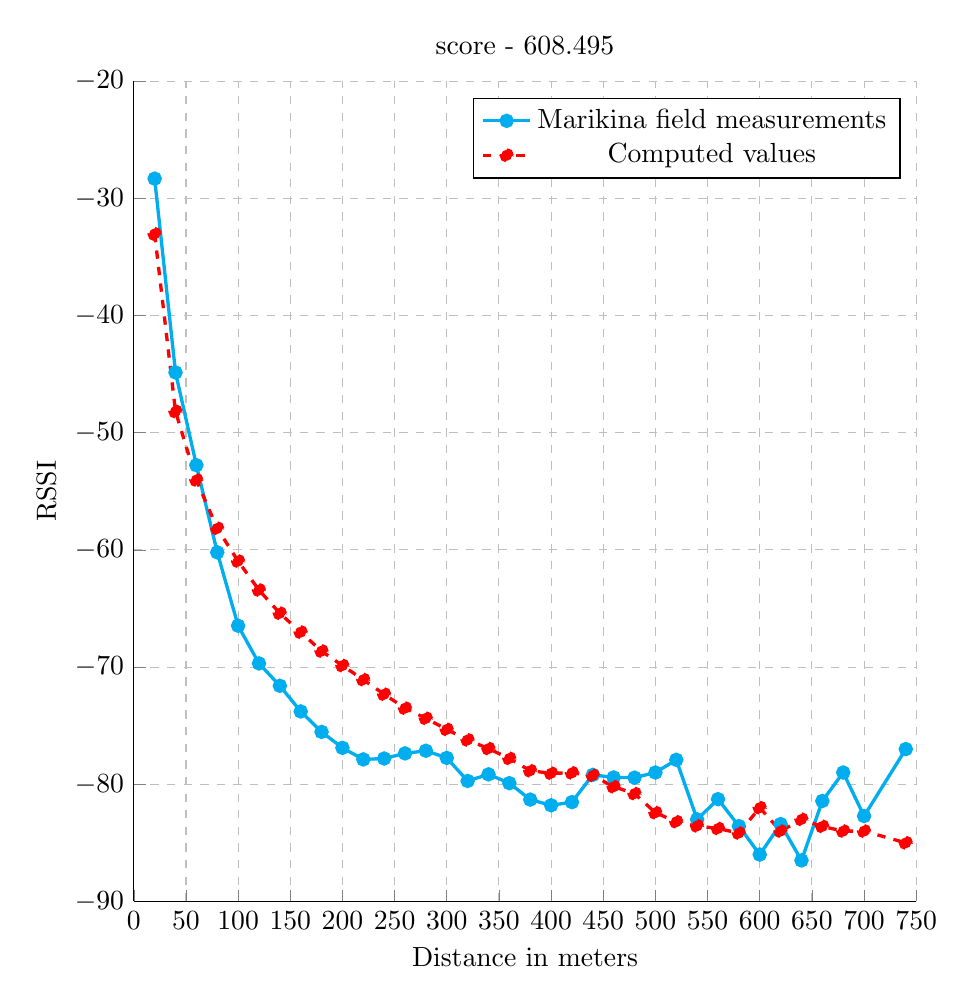
\begin{tikzpicture}%\label{plot:reachi-experiments:average-distance}
        \begin{axis}[
                title=score - 608.495,
                height=12cm, width=0.95\textwidth,
                ylabel={RSSI},
                xlabel={Distance in meters},
                axis lines*=left,
                xmin=0, xmax=750,
                enlargelimits=false,
                ymin=-90, ymax=-20,
                xtick={0, 50, 100, 150, 200, 250, 300, 350, 400, 450, 500, 550, 600, 650, 700, 750},
                ymajorgrids=true,
                xmajorgrids=true,
                grid style=dashed,
            ]

            \addplot[very thick, solid, cyan, mark=*] coordinates {(20, -28.32345013477089) (40, -44.85830258302583) (60, -52.77323717948718) (80, -60.21201657458563) (100, -66.47435897435898) (120, -69.68905472636816) (140, -71.5976496922216) (160, -73.7866473149492) (180, -75.53428571428572) (200, -76.89289392378991) (220, -77.88135593220339) (240, -77.8035019455253) (260, -77.36784140969164) (280, -77.14030612244898) (300, -77.75299760191847) (320, -79.71686746987952) (340, -79.15481171548117) (360, -79.90728476821192) (380, -81.30909090909091) (400, -81.79746835443038) (420, -81.52272727272727) (440, -79.2) (460, -79.42105263157895) (480, -79.4375) (500, -79.0) (520, -77.91666666666667) (540, -83.0) (560, -81.27272727272727) (580, -83.57142857142857) (600, -86.0) (620, -83.4) (640, -86.5) (660, -81.42857142857143) (680, -79.0) (700, -82.71428571428571) (740, -77.0)};
            \addlegendentry{Marikina field measurements};

            \addplot[very thick, dashed, red, mark=*] coordinates {(20,-33.04359925788497)(40,-48.19327731092437)(60,-54.03703703703704)(80,-58.16688567674113)(100,-60.96085858585859)(120,-63.43184421534937)(140,-65.41129831516353)(160,-67.02463054187191)(180,-68.64031007751937)(200,-69.87730061349693)(220,-71.07770961145194)(240,-72.32267441860465)(260,-73.50986842105263)(280,-74.37786259541984)(300,-75.32413793103449)(320,-76.22083333333333)(340,-76.95930232558139)(360,-77.8018018018018)(380,-78.84883720930233)(400,-79.06557377049181)(420,-79.03030303030303)(440,-79.25)(460,-80.21428571428571)(480,-80.8)(500,-82.42857142857143)(520,-83.2)(540,-83.55555555555556)(560,-83.77777777777777)(580,-84.16666666666667)(600,-82.0)(620,-84.0)(640,-83.0)(660,-83.6)(680,-84.0)(700,-84.0)(740,-85.0)};
            \addlegendentry{Computed values};
        \end{axis}
    \end{tikzpicture}
    \caption{Field measurements vs computed values}
    \label{plot:reachi-experiments:phili-log-vs-computed}
\end{figure}


\begin{figure}[H]
    \centering
    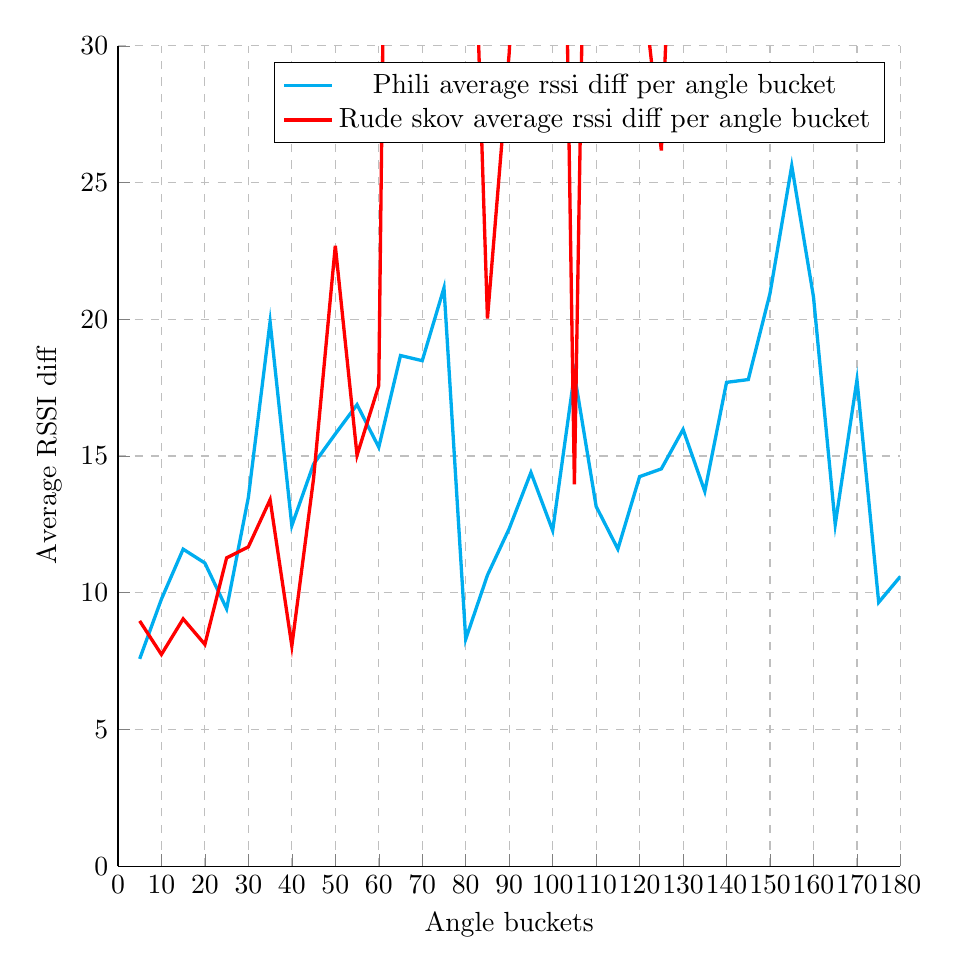
\begin{tikzpicture}%\label{plot:reachi-experiments:average-distance}
        \begin{axis}[
                height=12cm, width=0.95\textwidth,
                ylabel={Average RSSI diff},
                xlabel={Angle buckets},
                axis lines*=left,
                xmin=0, xmax=180,
                xtick={0, 10, 20, 30, 40, 50, 60, 70, 80, 90, 100, 110, 120, 130, 140, 150, 160,170,180},
                enlargelimits=false,
                ymin=0, ymax=30,
                ymajorgrids=true,
                xmajorgrids=true,
                grid style=dashed
            ]

            %\addplot[very thick, solid, cyan!50!black] coordinates {(5, 7.581215097994852) (10, 9.763581254686114) (15, 11.59234807189617) (20, 11.084399582147876) (25, 9.411670936293284) (30, 13.486232393853125) (35, 19.91110051641767) (40, 12.453590557884946) (45, 14.70313120243339) (50, 15.804939314638208) (55, 16.87697870999425) (60, 15.320902904198922) (65, 18.673392004683087) (70, 18.48508963612783) (75, 21.147550183881993) (80, 8.302184073487094) (85, 10.641508684206432) (90, 12.343183048128944) (95, 14.396643466792797) (100, 12.27504884861337) (105, 17.994872329043496) (110, 13.156645245862158) (115, 11.595967499573286) (120, 14.245146945189493) (125, 14.528392002600814) (130, 15.96981736460891) (135, 13.70427190114752) (140, 17.692009757218077) (145, 17.79486440192431) (150, 20.947579654378668) (155, 25.611175147469265) (160, 20.819124899373364) (165, 12.495568407794714) (170, 17.784042978338544) (175, 9.646875797269503) (180, 10.597197732034614)};
            \addplot[very thick, solid, cyan] coordinates {(5,7.581215097994852)(10,9.763581254686114)(15,11.59234807189617)(20,11.084399582147876)(25,9.411670936293284)(30,13.486232393853125)(35,19.91110051641767)(40,12.453590557884946)(45,14.70313120243339)(50,15.804939314638208)(55,16.87697870999425)(60,15.320902904198922)(65,18.673392004683087)(70,18.48508963612783)(75,21.147550183881993)(80,8.302184073487094)(85,10.641508684206432)(90,12.343183048128944)(95,14.396643466792797)(100,12.27504884861337)(105,17.994872329043496)(110,13.156645245862158)(115,11.595967499573286)(120,14.245146945189493)(125,14.528392002600814)(130,15.96981736460891)(135,13.70427190114752)(140,17.692009757218077)(145,17.79486440192431)(150,20.947579654378668)(155,25.611175147469265)(160,20.819124899373364)(165,12.495568407794714)(170,17.784042978338544)(175,9.646875797269503)(180,10.597197732034614)};
            \addlegendentry{Phili average rssi diff per angle bucket};


            %\addplot[very thick, solid, red!50!black] coordinates {(5, 8.968175725354994) (10, 7.741408675352775) (15, 9.042742837449076) (20, 8.108954051047618) (25, 11.273321343260399) (30, 11.67692967914715) (35, 13.401460743255232) (40, 8.053793318539391) (45, 14.17474549040368) (50, 22.68855220716477) (55, 15.026896145186285) (60, 17.5755161176863) (65, 85.01233086400362) (70, 59.69038212814202) (75, 62.41948703096457) (80, 44.72712810089782) (85, 20.029080610052482) (90, (29.737954905927445) (95, 43.39235466255519) (100, 64.720015835849) (105, 13.965589072181558) (110, 61.334883149884675) (115, 36.30455538419785) (120, 33.32223486902817) (125, 26.172354285886417) (130, 45.62355888699502) (135, 55.8474401182669) (140, 47.511612928722954) (145, 49.70429537245245) (150, 50.649080550831435) (155, 52.34402139529124) (160, 51.45218633523966) (165, 51.805898996936115) (170, 52.39131328924595) (175, 48.78102582759046) (180, 51.91529108595685)};
            \addplot[very thick, solid, red] coordinates {(5,8.968175725354994)(10,7.741408675352775)(15,9.042742837449076)(20,8.108954051047618)(25,11.273321343260399)(30,11.67692967914715)(35,13.401460743255232)(40,8.053793318539391)(45,14.17474549040368)(50,22.68855220716477)(55,15.026896145186285)(60,17.5755161176863)(65,85.01233086400362)(70,59.69038212814202)(75,62.41948703096457)(80,44.72712810089782)(85,20.029080610052482)(90,29.737954905927445)(95,43.39235466255519)(100,64.720015835849)(105,13.965589072181558)(110,61.334883149884675)(115,36.30455538419785)(120,33.32223486902817)(125,26.172354285886417)(130,45.62355888699502)(135,55.8474401182669)(140,47.511612928722954)(145,49.70429537245245)(150,50.649080550831435)(155,52.34402139529124)(160,51.45218633523966)(165,51.805898996936115)(170,52.39131328924595)(175,48.78102582759046)(180,51.91529108595685)};
            \addlegendentry{Rude skov average rssi diff per angle bucket};
        \end{axis}
    \end{tikzpicture}
    \caption{}
    \label{plot:reachi-experiments:avg-rssi-angle-phili-rude}
\end{figure}



\todo[inline]{show some plots, proving the problems}
\todo[inline]{talk about the visualiser + youtube link that shows the problems}
\todo[inline]{shortly mention CVPL and BOPL model that will be introduced in detail later}
\newpage
\section{Linkmodel}
In this section, our own Linkmodel will be described.

\subsection{Computing path loss}
To facilitate to the problems discussed in \autoref{sec:reachi-experiments}, we have devised our own linkmodel to compute path loss. Our model computes path loss based on the distance of the link and the percentage of that distance that is in a building. Building and other obstructions in the environment cause more severe path loss, and as such should be considered to punish the signal more. Our model limits to only buildings. The idea is to generate a map of the area that the nodes are located in as an image, then when computing the path loss of a link, look up the colour of all pixels in a straight line between the nodes  of link and count how many is a building. This gives a percentage for how much of the distance is covered by buildings. An pseudo code implementation of the computation can be seen on \autoref{algo:linkmodel:compute-building-percentage}.

\begin{algorithm}[H]
    \DontPrintSemicolon
    \SetKwFunction{FLoSModelCompute}{ComputeBuildingPercentage}
    \SetKwProg{Fn}{Function}{}{}

    \Fn{\FLoSModelCompute{$l$}}{
        $(n_1,\ n_2) \leftarrow \mathit{nodes}(l)$\;
        $(x_1,\ y_1) \leftarrow$ compute position for $n_1$\;
        $(x_2,\ y_2) \leftarrow$ compute position for $n_2$\;
        \;
        $\mathit{pixels} \leftarrow 0$\;
        $\mathit{buildings} \leftarrow 0$\;
        \While{$\lambda \in \{0 \dots 1\}$}{
            $(x,\ y) \leftarrow \lambda \cdot (x_1,\ y_1) + (1 - \lambda)\cdot(x_2,y_2)$\;
            \If{position ($x$, $y$) is a building}{
                $\mathit{buildings} \leftarrow \mathit{buildings} + 1$\;
            }
            $\mathit{pixels} \leftarrow \mathit{pixels} + 1$\;
        }

        \KwRet $\mathit{buildings} / \mathit{pixels}$\;
    }
    \caption{The ComputeBuildingPercentage function.}
    \label{algo:linkmodel:compute-building-percentage}
\end{algorithm}


We define two functions, $\mathit{cvpl(distance)}$ and $ \mathit{bopl(distance)}$. Both functions compute path loss based on distance. \gls{cvpl} computes path loss for distances with zero percent building, while \gls{bopl} computes path loss for 100\% building. When computing the path loss both functions will be used, in the following equation:
\todo[inline]{make me prettier}
\begin{eq}\label{eq:pl}
    \mathit{pl}(l) = (\mathit{cvpl}(d(l)) \cdot (1 - ComputeBuildingPercentage(l))) + (\mathit{bopl}(d(l)) \cdot ComputeBuildingPercentage(l))
\end{eq}

\todo[inline]{finish block}


\subsection{Approximating the constants}
\todo[inline]{rewrite as optimisation problem}
Finding the optimal constants for $\mathit{cvpl}$ and $\mathit{bopl}$ can defined as an optimisation problem. A set of links $L$ must be provided. The goal is to compute the difference from the computed \gls{rssi} to the measurements for all links in $L$.
\medbreak

The problem is defined as follows:
\begin{itemize}
    \item Input: A set of link $L$.
    \item Output: Optimal parameters for $\alpha,\ \beta,\ \delta$.
    \item Goal: Minimise the score function:\smallbreak
    $\mathit{compRSSI}(l)= \alpha \cdot (log_\delta(d(l))) + \beta$\smallbreak
    $\mathit{score}(\alpha, \beta, \delta) = \sum\limits_{l\ \in\ L} (\mathit{compRSSI}(l) - \mathit{measuredRSSI}(l))^2$

\end{itemize}

$\mathit{compRSSI}(l)$ is derived from $l_d$~\cite{paper:linkmodel}. As mentioned in \cite[p.~12]{paper:linkmodel}, $l_d$\'s constants are approximated based on the type of environment.\medbreak

To solve the optimisation problem, brute forcing will be utilised because of time restrictions. The set of links $L$, consisted of links with a computed building percentage below five percent or above 80\% was collected from the Marikina log into their separate collections. The Marikina log was used because the experiment was conducted in a city, resulting in links with varying building percentages. For both collections the links were further sorted based on distance of the links, with 20 meter intervals i.e. links with distances between 20 meters and 40 meters was sorted together. The average \gls{rssi} for each separation was then computed. Links with building percentage above 80\% was used for $\mathit{bopl}$ and links below 5 percent for $\mathit{cvpl}$. The parameters $\alpha,\ \beta \in \{-100 \dots 100\}$ with $0.5$ increments and $\delta\ \in \{2 \dots 100\}$ with $1$ increments. The result was the following functions:
\begin{eq}
    \mathit{cvpl}(l) = 48.5 \cdot (\ln{(d(l))} / \ln{(77)}) + 37.5
\end{eq}

\begin{eq}
    \mathit{bopl}(l) = 67 \cdot (\ln{(d(l))} / \ln{(57))} + 11.5
\end{eq}


\subsection{Evaluation}

The functions $\mathit{cvpl}$ and $\mathit{bopl}$ have been plotted on \autoref{plot:reachi-experiments:cvpl-vs-bopl}. $\mathit{bopl}$ does indeed result in greater path loss, however the plot also reveals that op to 100 meters $\mathit{bopl}$ computes a better \gls{rssi} compared to $\mathit{cvpl}$. To further examine this, each function has been plotted with their training set. $\mathit{cvpl}$ on \autoref{plot:reachi-experiments:marikina-log-below-5-pct} and $\mathit{bopl}$ can be seen on \autoref{plot:reachi-experiments:marikina-log-above-80-pct}.


\begin{figure}[H]
    \centering
    \begin{tikzpicture}
        \begin{axis}[
                height=12cm, width=0.95\textwidth,
                ylabel={RSSI},
                xlabel={Distance in meters},
                axis lines*=left,
                xmin=0, xmax=750,
                enlargelimits=false,
                ymajorgrids=true,
                xmajorgrids=true,
                grid style=dashed,
                restrict y to domain=-120:0,
                samples=700
            ]

            \addplot[domain=0:1000, very thick, solid, cyan] {26 - bopl(x)};
            \addlegendentry{\gls{bopl}};

            \addplot[domain=0:1000, very thick, dashed, red] {26 - cvpl(x)};
            \addlegendentry{\gls{cvpl}};
        \end{axis}
    \end{tikzpicture}
    \caption{Plot showing sampels drawn from \gls{cvpl} and \gls{bopl}}
    \label{plot:reachi-experiments:cvpl-vs-bopl}
\end{figure}


\newpage
\begin{figure}[H]
    \centering
    \begin{tikzpicture}
        \begin{axis}[
                title=score: 0.0372 - links: 13481,
                height=10cm, width=0.95\textwidth,
                ylabel={RSSI},
                xlabel={Distance in meters},
                axis lines*=left,
                xmin=0, xmax=750,
                enlargelimits=false,
                ymin=-90, ymax=-30,
                xtick={0, 50, 100, 150, 200, 250, 300, 350, 400, 450, 500, 550, 600, 650, 700, 750},
                ymajorgrids=true,
                xmajorgrids=true,
                grid style=dashed,
                samples=700
            ]

            \addplot[very thick, solid, cyan, mark=*] coordinates {(20, -36.01344537815126) (40, -48.361111111111114) (60, -54.93279022403259) (80, -62.40816326530612) (100, -68.14871794871794) (120, -60.85954712362301) (140, -71.69568452380952) (160, -74.36896551724138) (180, -73.93817204301075) (200, -75.09929078014184) (220, -73.38403041825094) (240, -75.43994413407822) (260, -77.69102990033223) (280, -77.31512605042016) (300, -75.7751937984496) (320, -78.60714285714286) (340, -78.38524590163935) (360, -78.52459016393442) (380, -77.34285714285714) (400, -80.96153846153847) (420, -81.03571428571429) (440, -80.41379310344827) (460, -74.18181818181819) (480, -79.9090909090909) (500, -79.75) (520, -77.56521739130434) (540, -81.23076923076923) (560, -78.9) (580, -85.0) (620, -82.5) (640, -82.33333333333333) (660, -82.4) (680, -77.5) (700, -85.4) (740, -77.0)};
            \addlegendentry{Marikina field measurements}


            \addplot[domain=0:740, very thick, solid, red] {26 - cvpl(x)};
            \addlegendentry{\gls{cvpl}};
        \end{axis}
    \end{tikzpicture}
    \caption{Field measurements with building percentage below five percent.}
    \label{plot:reachi-experiments:marikina-log-below-5-pct}
\end{figure}

\begin{figure}[H]
    \centering
    \begin{tikzpicture}
        \begin{axis}[
                title=score: 501.4932 - links: 377 ,
                height=10cm, width=0.95\textwidth,
                ylabel={RSSI},
                xlabel={Distance in meters},
                axis lines*=left,
                xmin=0, xmax=380,
                enlargelimits=false,
                ymin=-90, ymax=-30,
                ymajorgrids=true,
                xmajorgrids=true,
                grid style=dashed,
                samples=400
            ]

            \addplot[very thick, solid, cyan, mark=*] coordinates {(20, -32.56521739130435) (40, -50.607142857142854) (60, -52.15384615384615) (80, -64.85714285714286) (100, -49.5) (120, -65.76623376623377) (140, -69.38888888888889) (160, -72.05714285714286) (180, -69.3125) (200, -78.83333333333333) (220, -76.84) (240, -75.75) (260, -80.91666666666667) (280, -72.88888888888889) (300, -78.95238095238095) (320, -76.44444444444444) (340, -82.75) (380, -87.0)};
            \addlegendentry{Marikina field measurements};

            \addplot[domain=0:380, very thick, solid, red] {26 - bopl(x)};
            \addlegendentry{\gls{bopl}};
        \end{axis}
    \end{tikzpicture}
    \caption{Field measurements with building percentage above 80\%.}
    \label{plot:reachi-experiments:marikina-log-above-80-pct}
\end{figure}

With the found optimal parameters for $\mathit{cvpl}$, the resulting was score was 501.4932 for 13481 links. The average score for a single link is then $0.0372 = 501.4932 / 13481$. We consider this as good score, and as can be seen on \autoref{plot:reachi-experiments:marikina-log-below-5-pct}, the function fits the measurements.\medbreak

The $\mathit{bopl}$ however got worse result. The score per link was 0.9302 which is much larger compared to the score for $\mathit{cvpl}$. It is important to note that there was only 377 links in the training set for the $\mathit{bopl}$ function, which is wastly less compared to the 13481 links for the $\mathit{cvpl}$ function. Another reason for the lower precisision of $\mathit{bopl}$ is that the training set does not only consist of links with 100\% building, as we allowed for links with more than 80\%. This was however necessary as there was close to none links with 100\% building. Having a large set of links with 100\% building would result in higher precision.

\begin{figure}[H]
    \centering
    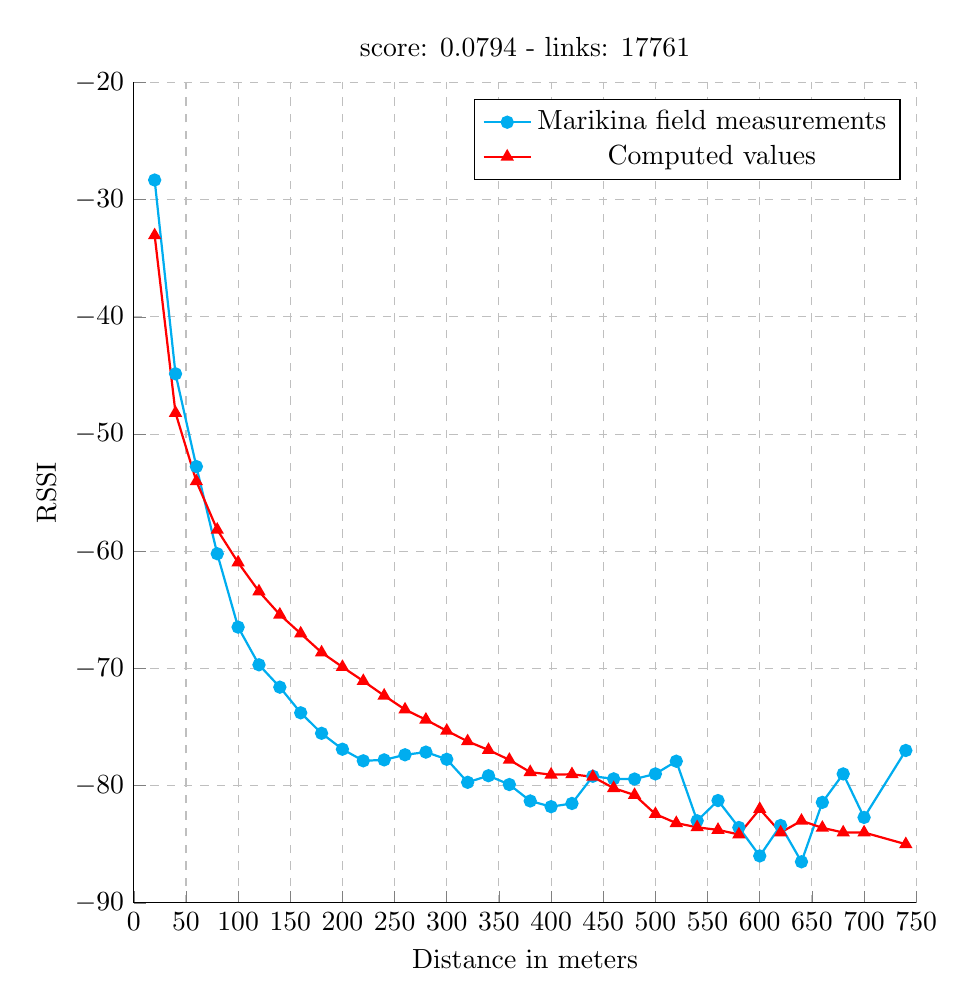
\begin{tikzpicture}
        \begin{axis}[
                title=score: 0.0794 - links: 17761,
                height=12cm, width=0.95\textwidth,
                ylabel={RSSI},
                xlabel={Distance in meters},
                axis lines*=left,
                xmin=0, xmax=750,
                enlargelimits=false,
                ymin=-90, ymax=-20,
                xtick={0, 50, 100, 150, 200, 250, 300, 350, 400, 450, 500, 550, 600, 650, 700, 750},
                ymajorgrids=true,
                xmajorgrids=true,
                grid style=dashed,
            ]

            \addplot[thick, solid, cyan, mark=*] coordinates {(20, -28.32345013477089) (40, -44.85830258302583) (60, -52.77323717948718) (80, -60.21201657458563) (100, -66.47435897435898) (120, -69.68905472636816) (140, -71.5976496922216) (160, -73.7866473149492) (180, -75.53428571428572) (200, -76.89289392378991) (220, -77.88135593220339) (240, -77.8035019455253) (260, -77.36784140969164) (280, -77.14030612244898) (300, -77.75299760191847) (320, -79.71686746987952) (340, -79.15481171548117) (360, -79.90728476821192) (380, -81.30909090909091) (400, -81.79746835443038) (420, -81.52272727272727) (440, -79.2) (460, -79.42105263157895) (480, -79.4375) (500, -79.0) (520, -77.91666666666667) (540, -83.0) (560, -81.27272727272727) (580, -83.57142857142857) (600, -86.0) (620, -83.4) (640, -86.5) (660, -81.42857142857143) (680, -79.0) (700, -82.71428571428571) (740, -77.0)};
            \addlegendentry{Marikina field measurements};

            \addplot[thick, solid, red, mark=triangle*] coordinates {(20,-33.04359925788497)(40,-48.19327731092437)(60,-54.03703703703704)(80,-58.16688567674113)(100,-60.96085858585859)(120,-63.43184421534937)(140,-65.41129831516353)(160,-67.02463054187191)(180,-68.64031007751937)(200,-69.87730061349693)(220,-71.07770961145194)(240,-72.32267441860465)(260,-73.50986842105263)(280,-74.37786259541984)(300,-75.32413793103449)(320,-76.22083333333333)(340,-76.95930232558139)(360,-77.8018018018018)(380,-78.84883720930233)(400,-79.06557377049181)(420,-79.03030303030303)(440,-79.25)(460,-80.21428571428571)(480,-80.8)(500,-82.42857142857143)(520,-83.2)(540,-83.55555555555556)(560,-83.77777777777777)(580,-84.16666666666667)(600,-82.0)(620,-84.0)(640,-83.0)(660,-83.6)(680,-84.0)(700,-84.0)(740,-85.0)};
            \addlegendentry{Computed values};
        \end{axis}
    \end{tikzpicture}
    \caption{Field measurements vs computed values}
    \label{plot:reachi-experiments:marikina-log-vs-computed}
\end{figure}


Finally a comparison of the computed results from \autoref{eq:pl} compared with the measurements from the Marikina log. Once again, links have been sorted into distance buckets and had the average \gls{rssi} for each bucket computed. The computed \gls{rssi}, was computed with \autoref{eq:pl} on the links from the Marikina log, but the field measured \gls{rssi} was removed. The computed \gls{rssi} was added instead, and the same sorting into distance buckets was done with the computed log. The result can be seen on \autoref{plot:reachi-experiments:marikina-log-vs-computed}. The computed score, once again, for a single link was 0.0794. \autoref{plot:reachi-experiments:marikina-log-vs-computed} shows that the function is off on the range from about 75 meters to 300 meters, however when compared with \autoref{plot:reachi-experiments:measurements-vs-ld} ours does indeed give a better result.
\section{Radio Simulation}\label{sec:radiomodel}
%\bibtodo{slight changes from original}
To simulate loss of packets during radio communication, we introduce the packet error probability. The packet
error probability is the probability for any form of error occurring during the transmission and reception of
a packet through wireless radio communication. The probability for packet error is calculated using the
\gls{rssi} on a link between two nodes, the size of the packet, as well as the \gls{snr}, including
interference from nearby transmitting nodes. The computations in this section are derived from
\cite{massoud2007digital}, as well as personal communication with the author of \cite{paper:linkmodel}.

\subsection{Probability for Packet Error}\label{sec:pep}
The first step for computing the probability for packet error is to compute the level of background noise
affecting the wireless communication, the noise power $P_{N,\mathit{dB}}$. This noise is calculated with the
thermal noise and noise figure $P_{N,\mathit{dB}} = \mathit{thermalnoise}\ +\ \mathit{noisefigure}$. For the
Reachi devices we assume that the $\mathit{thermalnoise} = -119.66$ \acrshort{db} and the
$\mathit{noisefigure} = 4.2$ \acrshort{db}. Next, we need to add the noise from interfering transmissions
happening at the same time. This is done by adding the sum of the \gls{rssi} from interfering transmitters to
the noise power $P_{N,\mathit{dB}}$, giving us the noise power with interference $P_{NI,\mathit{dB}}$ on the
specific link between a receiving node $n_r$ and a transmitting node $n_t$ at a given time $t$. The set of
currently transmitting and interfering nodes are denoted by $\mathit{nodes}_i$ and the the function
$\mathit{RSSI}_{\mathit{dBm}}(n, m, t)$ denotes the \gls{rssi}, in \acrshort{dbm}, on the link between nodes
$n$ and $m$ at time $t$. We assume the \gls{rssi} on a link to be reciprocated, which means that
$\mathit{RSSI}_{\mathit{dBm}}(n, m, t) = \mathit{RSSI}_{\mathit{dBm}}(m, n, t)$.

\begin{eq}\label{eq:noisepower}
    P_{NI,\mathit{dB}}(n_r, m_t, \mathit{nodes}_i, t) = 10 \log_{10}\left( 10^{\frac{P_{N,\mathit{dB}}}{10}} +
    \mathlarger{\sum}\limits_{m \in \mathit{nodes}_i}  10^{\frac{\mathit{RSSI}_{\mathit{dBm}}(n_r, m, t)}{10}}
    \right)
\end{eq}

Note that as both the noise power $P_{N,\mathit{dB}}$ and the \gls{rssi} is in \acrshort{db} (a logarithmic
scale), we first need to convert the values to a linear scale, before we can compute the sum of the background
noise and the interfering noise, and then finally convert the value back into a logarithmic scale. \medbreak

With the noise and interference power $P_{NI,\mathit{dB}}$, we can compute the \gls{snir},
$\gamma_{\mathit{dB}}$. The \gls{snir} compares the \gls{rssi} of the signal to the level of the background
noise, as well as the noise from interfering transmitters. The ratio is computed by subtracting the noise
power $P_{NI,\mathit{dB}}$ from the \gls{rssi} of a link.

\begin{eq}
    \gamma_{\mathit{dB}}(n_r, m_t, \mathit{nodes}_i, t) = \mathit{RSSI}_{\mathit{dBm}}(n_r, m_t, t) -
    P_{NI,\mathit{dB}}(n_r, m_t, \mathit{nodes}_i, t)
\end{eq}

We use the \gls{snir} $\gamma_{\mathit{dB}}$ to compute the bit error probability $P_b$:

\begin{eq}
    P_b(n_r, m_t, \mathit{nodes}_i, t) = \frac{1}{2}\mathit{erfc} \left( \sqrt{ \left(
    \frac{10^{\frac{\gamma_{\mathit{dB}}(n_r, m_t, \mathit{nodes}_i, t)}{10}}}{2} \right)} \right)
\end{eq}

Finally, with the bit error probability $P_b$, we can compute the packet error probability $P_p$. The packet
error probability is the probability that we experience a bit error for any of the bits in the transmitted
packet. The \textit{packetsize} parameter is in bytes.

\begin{eq}\label{eq:pep}
    P_p(n_r, m_t, \mathit{nodes}_i, \mathit{packetsize}, t) = 1 - \left( 1 - P_b(n_r, m_t, \mathit{nodes}_i,
    t) \right) ^{\mathit{packetsize} \cdot 8}
\end{eq}

\subsection{Example}
If we assume that a node $n_2$ is currently listening, and nodes $n_1$ and $n_3$ is transmitting at the same
time $t$, what is the probability for a packet error on the link between nodes $n_1$ and $n_2$ with
interference $\mathit{nodes}_i = \{ n_3 \} $? For this example we assume the \gls{rssi} for the link between
$n_1$ and $n_2$ to be $\mathit{RSSI}_{\mathit{dBm}}(n_2, n_1, t) = -63.750$, the \gls{rssi} between $n_2$ and
$n_3$ to be $\mathit{RSSI}_{\mathit{dBm}}(n_2, n_3, t) = -74.042$, and the size of the transmitted packet to
be 20 bytes (which is the size of a header packet for the Reachi protocol). First, we compute the noise power 
$P_{\mathit{NI}, \mathit{dB}}$:
\begin{eq}
    P_{\mathit{NI},\mathit{db}}(n_2, n_1, \mathit{nodes}_i, t) = 10 \log_{10}\left( 10^{\frac{(-119.66 + 4.2)}{10}} + 10^{\frac{-74.042}{10}} \right) = -74.041
\end{eq}

We subtract the noise power $P_{NI,dB}$ from the \gls{rssi} to get the \gls{snir} $\gamma_{dB}$:
\begin{eq}
    \gamma_{\mathit{dB}}(n_2, n_1, \mathit{nodes}_i, t) = -63.750 - (-74.041) = 10.291
\end{eq}

With which we can compute the bit error probability:
\begin{eq}
    P_b(n_2, n_1, \mathit{nodes}_i, t) = \frac{1}{2}erfc \left( \sqrt{ \left( \frac{10^{\frac{10.291}{10}}}{2} \right)} \right) = 0.000537
\end{eq}

Finally we can compute the packet error probability using the bit error probability:
\begin{eq}
    P_p(n_2, n_1, \mathit{nodes}_i, t, 20) = 1 - \left( 1 - 0.000537 \right) ^{20 \cdot 8} = 0.082
\end{eq}

This gives us an 8.2 \% probability that we will experience a packet error during the transmission from $n_1$
to $n_2$ with interference from $n_3$, which is a significant difference in relation to the same transmission
with no interfering transmitters. To demonstrate the difference, \autoref{plot:radiomodel:no-interference}
shows the probability for packet error with no interfering transmitters. According to the figure, an
\gls{rssi} of approximately $-103.0$ \acrshort{dbm} would have a probability for packet error close to zero,
and an \gls{rssi} of approximately $-110.0$ \acrshort{dbm} would have a probability for packet error very
close to 100.0 \%. Recall that for the link between $n_1$ and $n_2$ at time $t$, we had an \gls{rssi} of
$-63.750$ \acrshort{dbm}, which is significantly better than the $-103.0$ \acrshort{dbm} we see in
\autoref{plot:radiomodel:no-interference} for a close to zero probability, but with just a single interfering
transmitter, the probability for packet error increases to 8.2 \%, which corresponds to what we see in
\autoref{plot:radiomodel:one-interference}, where and \gls{rssi} of approximately $-62.0$ \acrshort{dbm} is 
required for a probability for packet error close to zero, with a single interfering transmitter.

\begin{figure}[H]
    \centering
    \begin{subfigure}[t]{.9\textwidth}
        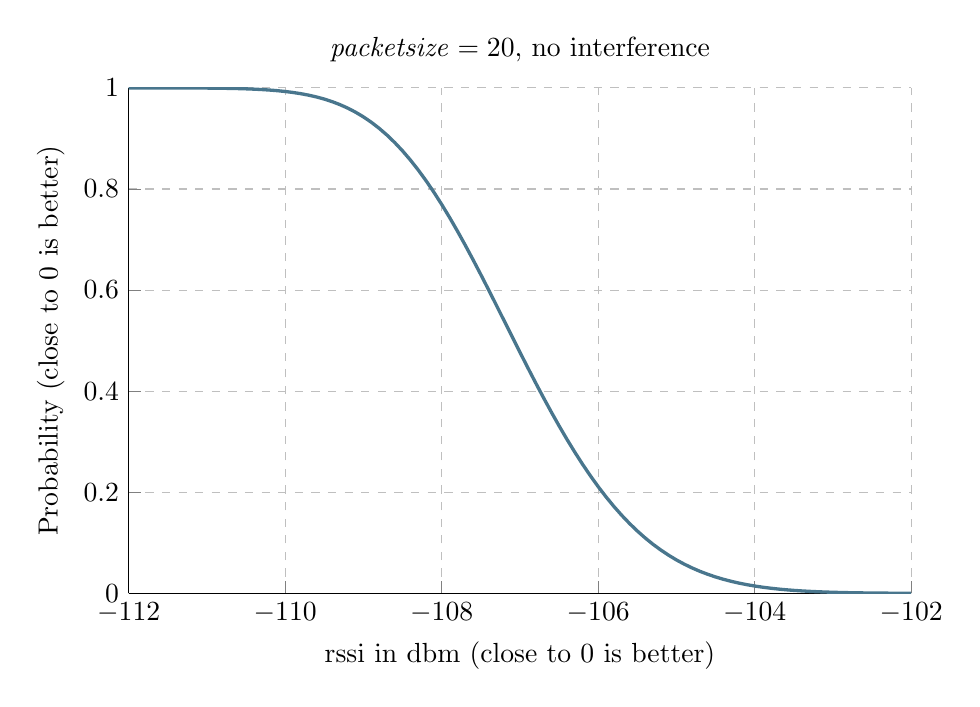
\begin{tikzpicture}%\label{plot:reachi-experiments:average-distance}
            \begin{axis}[
                    title={$\mathit{packetsize} = 20$, no interference},
                    height=8cm, width=0.95\textwidth,
                    ylabel={Probability (close to 0 is better)},
                    xlabel={\gls{rssi} in \acrshort{dbm} (close to 0 is better)},
                    axis lines*=left,
                    enlargelimits=false,
                    xtick={-112, -110, -108, -106, -104, -102},
                    ymajorgrids=true,
                    xmajorgrids=true,
                    grid style=dashed,
                ]
    
                \addplot[very thick, solid, cyan!50!black] coordinates {(-112,0.9999876428126551)(-111.9,0.9999818533805854)(-111.8,0.9999735236168629)(-111.7,0.9999616235974554)(-111.6,0.9999447451717537)(-111.5,0.999920980149257)(-111.4,0.9998877661533198)(-111.3,0.999841694145744)(-111.2,0.9997782714374498)(-111.1,0.9996916341768787)(-111.0,0.9995742039839494)(-110.9,0.999416284715221)(-110.8,0.9992055974422288)(-110.7,0.9989267547148308)(-110.6,0.9985606791379564)(-110.5,0.9980839762217061)(-110.4,0.9974682772917275)(-110.3,0.9966795747809701)(-110.2,0.995677579153797)(-110.1,0.9944151335993024)(-110.0,0.9928377289131765)(-109.9,0.9908831660120753)(-109.8,0.9884814165838162)(-109.7,0.9855547327690343)(-109.6,0.9820180538712832)(-109.5,0.977779751436127)(-109.4,0.9727427433945262)(-109.3,0.966805993404494)(-109.2,0.9598663934709013)(-109.1,0.9518210071670542)(-109.0,0.9425696284608098)(-108.9,0.9320175886859855)(-108.8,0.9200787232079811)(-108.7,0.9066783914790133)(-108.6,0.8917564310398185)(-108.5,0.8752699189322612)(-108.4,0.8571956138868371)(-108.3,0.8375319599914338)(-108.2,0.8163005472222238)(-108.1,0.7935469455391158)(-108.0,0.769340856001552)(-107.9,0.7437755528934127)(-107.8,0.7169666232111204)(-107.7,0.6890500419860338)(-107.6,0.6601796517461043)(-107.5,0.6305241401480931)(-107.4,0.6002636299578492)(-107.3,0.5695860091061149)(-107.2,0.5386831349945436)(-107.1,0.5077470465831848)(-107.0,0.4769663105493268)(-106.9,0.4465226148609678)(-106.8,0.4165877056515772)(-106.7,0.3873207426887495)(-106.6,0.35886612643390514)(-106.5,0.3313518270787408)(-106.4,0.3048882242599883)(-106.3,0.27956744643051556)(-106.2,0.25546318188223016)(-106.1,0.23263091968407745)(-106.0,0.21110856856704174)(-105.9,0.19091739506360728)(-105.8,0.17206321880579134)(-105.7,0.15453780245757087)(-105.6,0.13832037585666812)(-105.5,0.12337923806141704)(-105.4,0.10967338661475745)(-105.3,0.09715412994657713)(-105.2,0.08576664597225181)(-105.1,0.07545145721250357)(-105.0,0.06614579982676905)(-104.9,0.057784870567569646)(-104.8,0.050302941646255594)(-104.7,0.04363433873657152)(-104.6,0.037714281778700065)(-104.5,0.032479591872253466)(-104.4,0.027869270393728107)(-104.3,0.023824958598936963)(-104.2,0.0202912874470752)(-104.1,0.017216128297656508)(-104.0,0.014550755569625706)(-103.9,0.012249932504283412)(-103.8,0.010271930917551964)(-103.7,0.00857849534048738)(-103.6,0.007134761292770797)(-103.5,0.005909136667815562)(-103.4,0.004873154377310507)(-103.3,0.004001303543972212)(-103.2,0.003270845672304956)(-103.1,0.002661621391885305)(-103.0,0.00215585257009554)(-102.9,0.0017379438436174732)(-102.8,0.0013942869261214241)(-102.7,0.0011130704181615547)(-102.6,0.0008840972739669883)(-102.5,0.000698611570752572)(-102.4,0.0005491357749322079)(-102.3,0.0004293193051855271)(-102.2,0.00033379885272988297)(-102.1,0.0002580706275865374)(-102.0,0.0001983744574920454)};
    
            \end{axis}
        \end{tikzpicture}
       \caption{Probability for packet error on a link with no interfering transmitters.}\label{plot:radiomodel:no-interference}
    \end{subfigure}
    \begin{subfigure}[t]{.9\textwidth}
        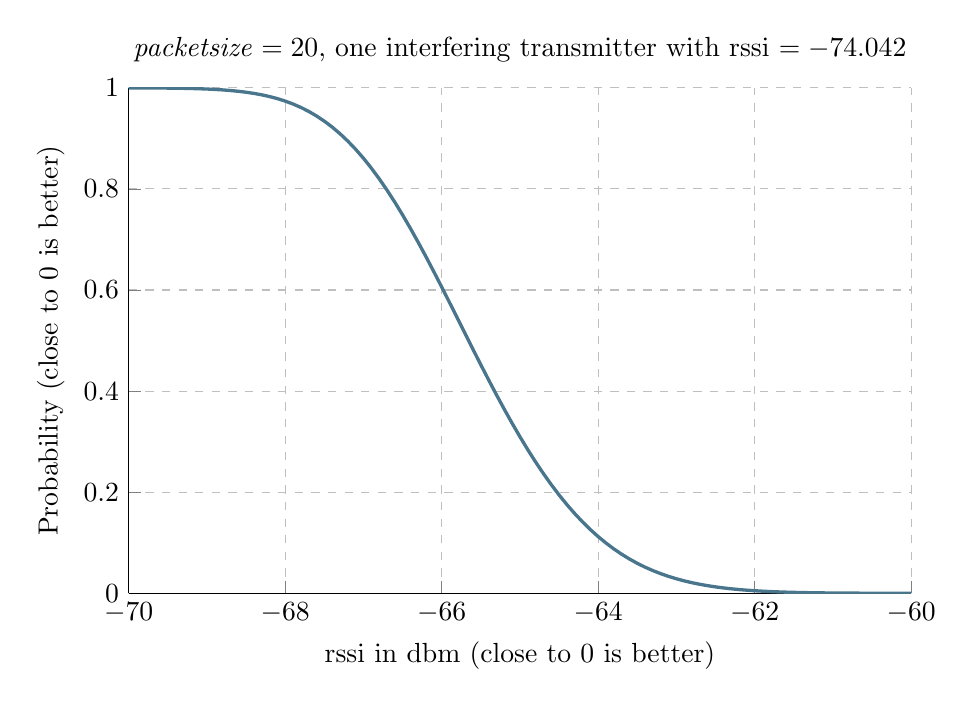
\begin{tikzpicture}%\label{plot:reachi-experiments:average-distance}
            \begin{axis}[
                 title={$\mathit{packetsize} = 20$, one interfering transmitter with \gls{rssi} $= -74.042$},
                    height=8cm, width=0.95\textwidth,
                    ylabel={Probability (close to 0 is better)},
                    xlabel={\gls{rssi} in \acrshort{dbm} (close to 0 is better)},
                    axis lines*=left,
                    enlargelimits=false,
                    xtick={-70, -68, -66, -64, -62, -60},
                    ymajorgrids=true,
                    xmajorgrids=true,
                    grid style=dashed,
                ]
                
                \addplot[very thick, solid, cyan!50!black] coordinates
                {(-70,0.9998946969201213)(-69.9,0.999851280175236)(-69.8,0.9997914288482014)(-69.7,0.9997095541645235)(-69.6,0.9995984200856673)(-69.5,0.9994487512548663)(-69.4,0.999248779311367)(-69.3,0.9989837280265265)(-69.2,0.9986352414918488)(-69.1,0.9981807643451096)(-69.0,0.997592888694345)(-68.9,0.9968386888236752)(-68.8,0.9958790716514758)(-68.7,0.9946681778438871)(-68.6,0.9931528749262344)(-68.5,0.9912723890419786)(-68.4,0.9889581254816121)(-68.3,0.9861337290346813)(-68.2,0.9827154329627786)(-68.1,0.9786127394483093)(-68.0,0.973729464463402)(-67.9,0.9679651661382458)(-67.8,0.9612169582453458)(-67.7,0.9533816900793851)(-67.6,0.9443584518788336)(-67.5,0.9340513423828241)(-67.4,0.9223724137305926)(-67.3,0.9092446903599295)(-67.2,0.894605144450226)(-67.1,0.8784075021721859)(-67.0,0.8606247535759753)(-66.9,0.841251244920013)(-66.8,0.8203042456090053)(-66.7,0.7978249020903394)(-66.6,0.7738785169287781)(-66.5,0.74855412125948)(-66.4,0.7219633410028916)(-66.3,0.6942385895436469)(-66.2,0.6655306499723479)(-66.1,0.6360057365895722)(-66.0,0.6058421466303818)(-65.9,0.5752266279786769)(-65.8,0.5443505964027997)(-65.7,0.5134063364756047)(-65.6,0.48258331425256296)(-65.5,0.4520647177980315)(-65.4,0.422024324919833)(-65.3,0.392623777345657)(-65.2,0.36401031848479315)(-65.1,0.33631502926640344)(-65.0,0.3096515746076566)(-64.9,0.2841154529163329)(-64.8,0.25978372350145207)(-64.7,0.2367151724125871)(-64.6,0.2149508663479005)(-64.5,0.19451503691409577)(-64.4,0.17541623353097346)(-64.3,0.1576486823314981)(-64.2,0.14119379008160704)(-64.1,0.1260217359331075)(-64.0,0.11209309920507793)(-63.9,0.09936047785157087)(-63.8,0.08777005934655302)(-63.7,0.07726311298604938)(-63.6,0.06777737973327802)(-63.5,0.05924834244541988)(-63.4,0.05161036543000741)(-63.3,0.04479769765769026)(-63.2,0.038745338542438446)(-63.1,0.03338976897292556)(-63.0,0.02866955326566123)(-62.9,0.024525819961693007)(-62.8,0.02090263097826983)(-62.7,0.017747249636844042)(-62.6,0.015010318608602913)(-62.5,0.012645958934183965)(-62.4,0.010611801070009363)(-62.3,0.008868958463135512)(-62.2,0.007381953529277174)(-62.1,0.006118605158747625)(-62.0,0.00504988605383716)(-61.9,0.004149757343889449)(-61.8,0.0033949870645402225)(-61.7,0.0027649582456965582)(-61.6,0.002241471548095064)(-61.5,0.0018085466304298414)(-61.4,0.0014522257270703776)(-61.3,0.0011603822729023827)(-61.2,0.0009225368308002357)(-61.1,0.0007296820553771566)(-61.0,0.0005741179660628815)(-60.9,0.0004492983977033571)(-60.8,0.0003496891470554653)(-60.7,0.0002706380340258274)(-60.6,0.00020825684500058728)(-60.5,0.0001593149176219999)(-60.4,0.00012114395831475111)(-60.3,9.15535532985956e-05)(-60.2,6.875673521467007e-05)(-60.1,5.130489908311553e-05)(-60.0,3.803131895474543e-05)};
    
            \end{axis}
        \end{tikzpicture}
       \caption{Probability for packet error on a link with a single interfering transmitter.}\label{plot:radiomodel:one-interference}
    \end{subfigure}
    \caption{Probability for packet error with and without interfering transmitters.}
    \label{figure:pepegraphs}
\end{figure}
